%% LyX 2.0.5.1 created this file.  For more info, see http://www.lyx.org/.
%% Do not edit unless you really know what you are doing.
\documentclass[english,11pt]{article}
\usepackage[T1]{fontenc}
\usepackage[latin9]{inputenc}
\usepackage{geometry}
\geometry{verbose,tmargin=1in,bmargin=1in,lmargin=1in,rmargin=1in}
\usepackage{babel}
\usepackage{amstext}
\usepackage{graphicx}
\usepackage[unicode=true,pdfusetitle,
 bookmarks=true,bookmarksnumbered=false,bookmarksopen=false,
 breaklinks=false,pdfborder={0 0 1},backref=false,colorlinks=false]
 {hyperref}

\makeatletter
%%%%%%%%%%%%%%%%%%%%%%%%%%%%%% User specified LaTeX commands.
\usepackage{ae,aecompl}

%\usepackage[normalmargins,normalbib,normaltitle,normalsections,normalindent]{savetrees}
%\usepackage[normalbib]{savetrees}

\providecommand{\onlinecite}{\cite}
\providecommand{\onlineref}{\ref}
\providecommand{\FToth}{Fejes T\'oth}

\makeatother

\begin{document}

\title{Mixed-Mode Instability in a Ternary Mixture}

\maketitle
\global\long\def\V#1{\boldsymbol{#1}}
\global\long\def\M#1{\boldsymbol{#1}}
\global\long\def\Set#1{\mathbb{#1}}


\global\long\def\D#1{\Delta#1}
\global\long\def\d#1{\delta#1}


\global\long\def\norm#1{\left\Vert #1\right\Vert }
\global\long\def\abs#1{\left|#1\right|}


\global\long\def\grad{\M{\nabla}}
\global\long\def\avv#1{\langle#1\rangle}
\global\long\def\av#1{\left\langle #1\right\rangle }


\global\long\def\ki{k}
\global\long\def\wi{\omega}


This is a summary of the experimental setup from \cite{MixedDiffusiveInstability}
for getting a nice diffusion-driven gravitational instability in a
simple ternary mixture: a solution of sugar on top of a solution of
salt (in the beginning the density should be higher on the bottom
so it starts off stable). I suggest our target to be to reproduce
some aspects (at least the pretty picture) in Fig. 4 of \cite{MixedDiffusiveInstability}
-- this is the mixed-mode instability. This is when one starts with
an unstable (heavy on top of light fluid) situation but the differential
diffusion effects also affect the instability. One can also consider
the simpler DLC instability (we did this in the PRE for compressible
flow) or the classical salt-fingering DD instability, but the mixed-mode
one seems most interesting and complex.

\begin{figure}
\begin{centering}
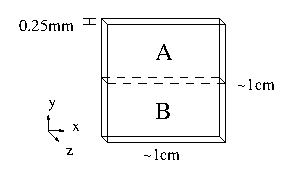
\includegraphics[width=1\textwidth]{mmi}
\par\end{centering}

\caption{MMI}
\end{figure}


We consider a ternary mixture of salt (KCl, species 1, molar mass
$74.55\, g\text{�}mol^{-1}$, denoted by A in paper), sugar (sucrose,
species 2, molar mass $342.3\, g\text{�}mol^{-1}$, denoted by B in
paper) and water (species 3, molar mass $18.02\, g\text{�}mol^{-1}$).
The initial configuration is salt solution on top of sugar solution.

Our equation of state is defined as

\begin{equation}
\sum_{i}\frac{\rho_{i}}{\bar{\rho}_{i}}=\rho\sum_{i}\frac{w_{i}}{\bar{\rho}_{i}}=1,\label{eq:EOS}
\end{equation}
where $w_{i}=\rho_{i}/\rho$ is the mass fraction and $\bar{\rho}_{i}$
are the (potentially ficticious) pure component densities. We can
write this in the form
\begin{equation}
\frac{\rho-\rho_{1}-\rho_{2}}{\bar{\rho}_{3}}+\frac{\rho_{1}}{\bar{\rho}_{1}}+\frac{\rho_{2}}{\bar{\rho}_{2}}=1.\label{eq:eos_1}
\end{equation}
In the paper, the approximate formula for the density is
\begin{equation}
\rho=\rho_{0}\left(1+\alpha_{1}Z_{1}+\alpha_{2}Z_{2}\right)=\rho_{0}\left(1+\frac{\alpha_{1}}{M_{1}}\rho_{1}+\frac{\alpha_{2}}{M_{2}}\rho_{2}\right),\label{eq:eos_2}
\end{equation}
where $\rho_{0}=\bar{\rho}_{3}=10^{3}\, g/l$ (I use liter here since
they use it in the paper, we can use $cm^{3}$ in the actual runs)
is the density of water, $\alpha_{k}$ are constants and $Z_{k}$
is the number of moles of each component, related to the partial density
via $\rho_{k}=Z_{k}M_{k},$ where $M_{k}$ is the molar mass. By comparing
(\ref{eq:eos_1}) and (\ref{eq:eos_2}) we get
\[
1-\frac{\rho_{0}}{\bar{\rho}_{k}}=\rho_{0}\frac{\alpha_{k}}{M_{k}},
\]
which now gives us the value of 
\[
\bar{\rho}_{1}=2.81\text{ and }\bar{\rho}_{2}=1.55
\]
from the values of $\alpha$ tabulated in table I of the paper, $\alpha_{1}=4.8\cdot10^{-2}\, l/mol$
for KCl and $\alpha_{2}=12.2\cdot10^{-2}\, l/mol$ for sucrose. BTW,
when used for glycerol ($\alpha=2.3$ from Table I and molar mass
$92.2$), this gives $\bar{\rho}=1.33$, which is close to the correct
value of 1.26, as it should since glycerol exists as an actual liquid
pure phase.

For the diffusion coefficients, these mixtures are at what can be
considered ``infinite dilution'' so there is essentially no coupling
between the different components (from this pespective it is a bit
boring). In this limit the approximation proposed in \cite{Diffusion_InfiniteDilution}
suggest setting the Maxwell-Stefan diffusion coefficients to
\[
D_{13}=D_{1},\, D_{23}=D_{2},\, D_{12}=\frac{D_{1}D_{2}}{D_{3}},
\]
where from table I we read the self-diffusion coefficient of low-dilution
KCl in water as $D_{1}=1.91\cdot10^{-5}\, cm^{2}/s$, and for sucrose
$D_{2}=0.52\cdot10^{-5}\, cm^{2}/s$. Here $D_{3}$ is the self-diffusion
coefficient of pure water, $D_{3}=2.3\cdot10^{-5}\, cm^{2}/s$.

The initial concentrations on the top and bottom are determined from
the dimensionless number
\[
R=\frac{\alpha_{2}Z_{2}}{\alpha_{1}Z_{1}}=0.89.
\]
The initial values of the concentrations were reported to us to be
\[
Z_{1}^{0}=0.29\text{ and }Z_{2}^{0}=0.1\, mol/l,
\]
which gives initial densities differing by about $0.17\%$, 
\begin{eqnarray}
\rho_{\text{top}} & = & \rho_{0}\left(1+\alpha_{1}Z_{1}^{0}\right)=\left(1.0+4.8\cdot10^{-2}\times0.29\right)\, g/cm^{3}=1.0139\, g/cm^{3},\label{eq:ics}\\
\rho_{\text{bottom}} & = & \rho_{0}\left(1+\alpha_{2}Z_{2}^{0}\right)=\left(1.0+12.2\cdot10^{-2}\times0.1\right)\, g/cm^{3}=1.0122\, g/cm^{3},\nonumber 
\end{eqnarray}
which are not quite consistent with the the densities reported to
us, $\rho_{\text{top}}=1.0125\, g/cm^{3}$ and $\rho_{\text{bottom}}=1.0119\, g/cm^{3}$,
which differ by about $0.06\%$. In terms of the partial densities
of the two components we have
\[
\rho_{1}^{0}=Z_{1}^{0}M_{1}=0.0216\, g/cm^{3},\quad\rho_{2}^{0}=Z_{2}^{0}M_{2}=0.0342\, g/cm^{3},
\]
which are also very close to the initial mass fractions since the
total density is very close to $1\, g/cm^{3}$.

Lacking better experimental data and more consistent response from
the experimentalists, for the final simulations reported in the paper
we use four times larger concentrations; this preserves the dimensionless
number $R$ which is presumed to be the most important number. Specifically,
we set the initial mass fractions to
\[
w_{1}^{0}=0.0864,\quad w_{2}^{0}=0.1368,
\]
which from the EOS gives
\begin{eqnarray*}
\rho_{\text{top}} & = & \left(\frac{0.0864}{2.81}+\frac{0.9136}{1.0}\right)^{-1}=1.0596\, g/cm^{3}\\
\rho_{\text{bottom}} & = & \left(\frac{0.1368}{1.55}+\frac{0.8632}{1.0}\right)^{-1}=1.0510\, g/cm^{3}
\end{eqnarray*}
for a density difference of about 0.8\%.The plots in the bottom panel
of Fig. 1 are for times $40,50,60\, s,$ so we run our simulations out to
$60\, s.$  We use a geometry of $0.8cm^{2}$ in the $x-y$ plane (gravity along $y$
here), to nearly match the size of the snapshots in Fig. 1. The thickness
in the $z$ direction is $0.25mm$ (so \emph{very} thin).
Our computational domain is $256\times 256\times 8$ zones and we use a time
step limited by a diffusive mass CFL of 0.75, i.e.,
$\Delta t = 0.75 \Delta x^2 / (6 * D_{\rm max}) = 0.75 * .003125^2 / (6 * 1.91\times 10^{-5}) = 6.39\times 10^{-2}s$.
We are using the inertial code, as the overdamped code has trouble converging
at this aspect ratio.
Note that the
momentum diffusion time across $1cm$ length is 
$\tau_{\nu}\sim1cm^{2}/2\cdot10^{-2}\left(cm^{2}/s\right)\sim50s$.
We can use periodic BCs along $x$, and reservoir along $y$ (with
reservoir values set equal to the initial values), and no-slip along
$z$. They use some special experimental procedure to get a very flat
interface at the beginning, not sure however how close to a jump profile
it is (with bds advection we can do a jump also). They state the wavelength
of the Y-shaped instability fingers they get is on the order of $1.3mm$,
which is an important number to observe. To start off the instability
in deterministic simulations we can make the concentrations random
in the middle layer of cells like we did for the Kevin-Helmholtz instability.
The alternative is to use a flat interface and allow for thermal fluctuations
to set off initial perturbations.

%\bibliographystyle{unsrt}
%\bibliography{References,GarciaGeneralBibFile,MScaleProp}
\begin{thebibliography}{1}

\bibitem{MixedDiffusiveInstability}
Jorge Carballido-Landeira, Philip~MJ Trevelyan, Christophe Almarcha, and Anne
  De~Wit.
\newblock Mixed-mode instability of a miscible interface due to coupling
  between rayleigh-taylor and double-diffusive convective modes.
\newblock {\em Physics of Fluids}, 25(2):024107, 2013.

\bibitem{Diffusion_InfiniteDilution}
Xin Liu, Andre\u0301 Bardow, and Thijs~JH Vlugt.
\newblock Multicomponent maxwell- stefan diffusivities at infinite dilution.
\newblock {\em Industrial \& Engineering Chemistry Research}, 50(8):4776--4782,
  2011.

\end{thebibliography}

\end{document}
